\begin{titlepage}
  % HACK for two-sided documents: ignore binding correction for cover page.
  % Adapted from Markus Kohm's KOMA-Script titlepage=firstiscover handling.
  % See http://mirrors.ctan.org/macros/latex/contrib/koma-script/scrkernel-title.dtx,
  % \maketitle macro.
  \oddsidemargin=\evensidemargin\relax
  \textwidth=\dimexpr\paperwidth-2\evensidemargin-2in\relax
  \hsize=\textwidth\relax

  \centering

  % TODO: if you wish to remove the university logo
  % just delete the file logos/tum_logo.png
  \IfFileExists{logos/tum_logo.png}{
    
\includegraphics[width=4cm, height=20mm]{logos/tum_logo.png}
  }{
    \vspace*{20mm}
  }

  \vspace{5mm}
  {\huge\MakeUppercase{\getUniversity{}}}\\

  \vspace{5mm}
  {\large\MakeUppercase{\getFaculty{}}}\\

  \vspace{20mm}
  {\Large \getDoctype{}}

  \vspace{15mm}
  {\huge\bfseries \getTitle{}}

  \vspace{15mm}
  {\LARGE \getAuthor{}}

  % TODO: if you wish to remove the faculty logo
  % just delete the file logos/informatics_logo.png
  \IfFileExists{logos/informatics_logo.png}{
    \vspace{15mm}
    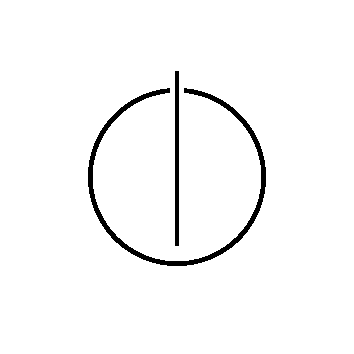
\includegraphics[height=60mm]{logos/informatics_logo.png}
  }{}
\end{titlepage}
